\documentclass[twoside]{article}
\setlength{\oddsidemargin}{0.25 in}
\setlength{\evensidemargin}{-0.25 in}
\setlength{\topmargin}{-0.6 in}
\setlength{\textwidth}{6.5 in}
\setlength{\textheight}{8.5 in}
\setlength{\headsep}{0.75 in}
\setlength{\parindent}{0 in}
\setlength{\parskip}{0.1 in}

\usepackage{graphicx}
\usepackage{url}
\usepackage{amsmath}

%
% The following commands sets up the lecnum (lecture number)
% counter and make various numbering schemes work relative
% to the lecture number.
%
\newcounter{lecnum}
\renewcommand{\thepage}{\thelecnum-\arabic{page}}
\renewcommand{\thesection}{\thelecnum.\arabic{section}}
\renewcommand{\theequation}{\thelecnum.\arabic{equation}}
\renewcommand{\thefigure}{\thelecnum.\arabic{figure}}
\renewcommand{\thetable}{\thelecnum.\arabic{table}}
\newcommand{\dnl}{\mbox{}\par}

%
% The following macro is used to generate the header.
%
\newcommand{\lecture}[4]{
  \pagestyle{myheadings}
  \thispagestyle{plain}
  \newpage
  \setcounter{lecnum}{#1}
  \setcounter{page}{1}
  \noindent
  \begin{center}
  \framebox{
     \vbox{\vspace{2mm}
   \hbox to 6.28in { {\bf COMPSCI~590S~~~Systems for Data Science
                       \hfill Fall 2016} }
      \vspace{4mm}
      \hbox to 6.28in { {\Large \hfill Lecture #1: #2  \hfill} }
      \vspace{2mm}
      \hbox to 6.28in { {\it Lecturer: #3 \hfill Scribe(s): #4} }
     \vspace{2mm}}
  }
  \end{center}
  \markboth{Lecture {#1}: #2}{Lecture {#1}: #2}
  \vspace*{4mm}
}

%
% Convention for citations is authors' initials followed by the year.
% For example, to cite a paper by Leighton and Maggs you would type
% \cite{LM89}, and to cite a paper by Strassen you would type \cite{S69}.
% (To avoid bibliography problems, for now we redefine the \cite command.)
%
\renewcommand{\cite}[1]{[#1]}

% \input{epsf}

%Use this command for a figure; it puts a figure in wherever you want it.
%usage: \fig{NUMBER}{FIGURE-SIZE}{CAPTION}{FILENAME}
\newcommand{\fig}[4]{
           \vspace{0.2 in}
           \setlength{\epsfxsize}{#2}
           \centerline{\epsfbox{#4}}
           \begin{center}
           Figure \thelecnum.#1:~#3
           \end{center}
   }

% Use these for theorems, lemmas, proofs, etc.
\newtheorem{theorem}{Theorem}[lecnum]
\newtheorem{lemma}[theorem]{Lemma}
\newtheorem{proposition}[theorem]{Proposition}
\newtheorem{claim}[theorem]{Claim}
\newtheorem{corollary}[theorem]{Corollary}
\newtheorem{definition}[theorem]{Definition}
\newenvironment{proof}{{\bf Proof:}}{\hfill\rule{2mm}{2mm}}

% Some useful equation alignment commands, borrowed from TeX
\makeatletter
\def\eqalign#1{\,\vcenter{\openup\jot\m@th
 \ialign{\strut\hfil$\displaystyle{##}$&$\displaystyle{{}##}$\hfil
     \crcr#1\crcr}}\,}
\def\eqalignno#1{\displ@y \tabskip\@centering
 \halign to\displaywidth{\hfil$\displaystyle{##}$\tabskip\z@skip
   &$\displaystyle{{}##}$\hfil\tabskip\@centering
   &\llap{$##$}\tabskip\z@skip\crcr
   #1\crcr}}
\def\leqalignno#1{\displ@y \tabskip\@centering
 \halign to\displaywidth{\hfil$\displaystyle{##}$\tabskip\z@skip
   &$\displaystyle{{}##}$\hfil\tabskip\@centering
   &\kern-\displaywidth\rlap{$##$}\tabskip\displaywidth\crcr
   #1\crcr}}
\makeatother

% **** IF YOU WANT TO DEFINE ADDITIONAL MACROS FOR YOURSELF, PUT THEM HERE:



% Some general latex examples and examples making use of the
% macros follow.

\begin{document}

%FILL IN THE RIGHT INFO.
%\lecture{**LECTURE-NUMBER**}{**DATE**}{**LECTURER**}{**SCRIBE**}
\lecture{3}{Parallelism}{Emery Berger}{Jun Wang,Omar Ismail}

\section{Terminology}
\emph{Speedup} is an important metric measuring the performance of parallelism. It compares the latency for solving the identical computational problem on one processor versus on $N$ processors:
\begin{equation}
\textnormal{speedup}(N) = \frac{T_1}{T_N},
\end{equation}
where $T_1$ is the latency, the time it takes to complete a task, of the program with one processor and $T_N$ is the latency on $N$ processors. In other words, $T_1$ is serial execution time, and $T_N$ is the parallel execution time. 

A speedup of more than $N$ with $N$ processors is called \emph{super-linear speedup}.
\emph{Embarrassingly parallel} is another case, which means when solving multiple independent task, little or no coordination between tasks is needed.

When introducing parallelism, a straight-forward question is that if parallelism can increase speedup unlimitedly. The quite answer is no. To deliberate this question, we introduce \emph{critical path length}, which is length of the event path in the execution history of the program that has the longest duration. Alternatively, it is the parallel execution time with infinite processor, so we denote it as $T_\infty$. 
Fig-\ref{cpl} shows a system with $100$ parallel tasks. Each circle is a task with latency of $1$ time unit. In this system,
$$
\textnormal{speedup}(100) = \frac{T_1}{T_{100}} = \frac{102}{3},
$$
and the parallel execution time is lower bounded by $3$ even with infinite processors.

\begin{figure}[h]
\centering
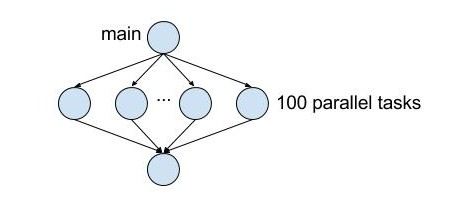
\includegraphics[width=0.5\linewidth]{fig1}
\caption[]{A system with 100 parallel tasks}
\label{cpl}
\end{figure}

Mathematically, speedup with $N$ processors is upper bounded as
\begin{equation}
	\textnormal{speedup}(N)\leq \frac{T_1}{T_\infty + \frac{T_1 - T_\infty}{N}}.
\end{equation}

\section{Performance theories}
Amdahl's law and Gustafson's law are two performance theories illustrating the trade-offs of parallel optimization.
\subsection{Amdahl's law}
Amdahl argued that the execution time $T_1$ falls into two categories:
\begin{itemize}
	\item Time spent doing non-parallelizable serial work, denoted as $s$
	\item Time spent doing parallelizable work, denoted as $p$
\end{itemize}
Then, 
\begin{eqnarray}
T_1 = s + p\\
T_N = s + p/N
\end{eqnarray}
and Amdahl's law states that
\begin{equation}
\textnormal{speedup}(N)\leq \frac{s+p}{s+p/N}.
\end{equation}

Amdahl's law indicates that speedup is limited by the fraction of the work that is not parallelizable even using infinity number of processors. It consists with our observation is last section.

\subsection{Gustafson's law}
Gustafson provides a more optimistic point of view.
Different from Amdahl,Gustafson disputed that in really, the workload is not constant; the work for parallel part scales with more processors. For example, if the completion time of a program is accelerated from $100$ seconds to $1$ second, then the more $99$ seconds should be utilized for more work.

Gustafson's law states that
\begin{equation} \label{eq1}
\begin{split}
\textnormal{scaled speedup}(N) & = \frac{s+ pN}{s+p} \\
& = s + pN\\
& = N + (1-N)s
\end{split}
\end{equation}
Gustafson's law is limited by the assumptions that serial work grows much more slowly than parallel work.

\section{Parallelism/super-linear}

Achieving super-linear results from parallelism is possible because of different factors. If you have 1.5GB of data to work with and only 1 GB of memory, one machine will have to hit the disk to finish processing, which takes more time. But if you have two machines (each with 1GB of memory) vs one machine, that means you can fit all the data (1.5GB) in memory (.75GB in each machine), which is much faster than looking at disk for data. So this achieves super-linear processing. 

The important thing to note is that the equations above from Amdhal's law and Gustafson's law are overly simplified, and should only be used as rough estimations and reference points. They ignore things like memory.

One of the goals of data science is to fit the work/data in RAM. There is a concept of a "working set" which is 'what stuff/data are you working on now?'.


\section{Garbage Collection}

Garbage collection is the mechanism in a programming language for cleaning out objects in the memory that have no pointers referencing/pointing to it — unreachable objects.

Some collectors have a "stop the world" approach, where they freeze everything and clean up unreachable objects. Other collectors do clean up unreachable objects concurrently. 

One way is to keep a reference count: keep track of the count of objects that have another pointing to it. The issue with this is cycles: where you have two objects pointing to each other but nothing else pointing to either of the two objects.


Another technique is to use Recursive Marking. That is a graph traversal of white/black marking of objects to see if there are any pointers. If white, remove, if black, then keep.

The amount of memory you use is a fraction of the total memory because the other
portion is used by garbage collector. Works like real life garbage.  You
wouldn’t go to dump every time you want to throw away one wrapper. Instead you wait till cans are full, then you go once.

Increasing performance of garbage collecting is a skill in and of itself. You can use a profiler to figure out how much memory you need to get it faster. If fast enough, then you are good. If not, then you have to dig into performance issues and use a variety of techniques to improve the garbage collecting. Performance of program depends on disk, RAM, what kind of data, etc. You cannot tell performance analytically, can only tell empirically.


\bibliographystyle{plain}
\bibliography{references}

\end{document}
